\documentclass[journal]{IEEEtran}
% *** GRAPHICS RELATED PACKAGES ***
%
\ifCLASSINFOpdf
   \usepackage[pdftex]{graphicx}
  % declare the path(s) where your graphic files are
   \graphicspath{{../pdf/}{../jpeg/}{./png/}}
  % and their extensions so you won't have to specify these with
  % every instance of \includegraphics
   \DeclareGraphicsExtensions{.pdf,.jpeg,.png}
\else
  % or other class option (dvipsone, dvipdf, if not using dvips). graphicx
  % will default to the driver specified in the system graphics.cfg if no
  % driver is specified.
   \usepackage[dvips]{graphicx}
  % declare the path(s) where your graphic files are
   \graphicspath{{../eps/}}
  % and their extensions so you won't have to specify these with
  % every instance of \includegraphics
   \DeclareGraphicsExtensions{.eps}
\fi

% *** MATH PACKAGES ***
%
\usepackage[cmex10]{amsmath}
\usepackage{stfloats}

\begin{document}

\title{Group 2 Final Project Report (revA1218)}
\author{Jay Guild, Nathan Miller, Matthew L Weber}

% The paper headers
\markboth{IOWA STATE UNIVERSITY - CPRE583, Fall 2013}%
{Shell \MakeLowercase{\textit{et al.}}: Bare Demo of IEEEtran.cls for Journals}
% The only time the second header will appear is for the odd numbered pages
% after the title page when using the twoside option.
% 
% *** Note that you probably will NOT want to include the author's ***
% *** name in the headers of peer review papers.                   ***
% You can use \ifCLASSOPTIONpeerreview for conditional compilation here if
% you desire.

\maketitle

\begin{abstract}
%\boldmath
This project seeks to characterize the acceleration of a Linux Kernel cryptography algorithm using programmable logic. It targets a specific algorithm and uses a combination of open source user space applications, new kernel drivers, and custom logic to create a working SoC FPGA design.
\end{abstract}

% Note that keywords are not normally used for peerreview papers.
%\begin{IEEEkeywords}
%\end{IEEEkeywords}

\IEEEpeerreviewmaketitle

\section{Introduction}
\IEEEPARstart{A}{cceleration} of a cryptographic algorithms on an embedded device remains an outstanding challenge. New System on Chip (SoC) FPGA technologies provide more options to offload or accelerate the cryptographic computations, however, integrating these technologies into existing designs can be challenging. Similarly, migrating designs between different SoC FPGA platforms can also require a significant investment of time and resources. Even though the system functionality and underlying algorithms remain unchanged, the design teams are forced to re-invent their designs for each new platform.

This project sought to characterize the effort of porting a simple cryptographic algorithm to a SoC FPGA prototype containing a fabric based accelerator and provide empirical performance data showing the benefits of doing so. Towards this end, we implemented the SHA-1 algorithm on a Xilinx Zynq SoC FPGA 702 development kit and compared the performance of our SHA-1 fabric to a pure software implementation running on the Zynq’s ARM core.  The Linux cryptodev framework provided transparent access to the SHA-1 function, permitting the user-space to be ignorant of where the SHA-1 function was actually being performed.   Our project uses similar concepts implemented on Texas Instruments SoC processors to tie their hardware accelerators into the Linux Kernel.

It would be fair to characterize our project as more of an “engineering project”.  Experimental data was certainly collected and analyzed (see the section VI \& VII), but the bulk of our effort was directed towards creating a working implementation.

\section{Related Work}
Cryptography is the process of encrypting information using an algorithm and either a public key (asymmetric encryption) or a private key (symmetric encryption) that makes the information unreadable unless the data is passed through a decryption algorithm that utilizes a private key that only the receiver holds\cite{HIPPA}. Several keys and algorithms have been developed under the IEEE standard for public key cryptography \cite{IEEESTD} and studied in several different environments for effectiveness and speed. It has been found that over networks with cryptography implemented that the limiting factor for most systems in speed is the network itself so using software to handle cryptography has not helped to speed up processing time much \cite{GUTMANN}. With speeds always increasing on communication buses this will change soon though. The largest bonuses in the recent past have been seen when adding a co-processor or FPGA to handle cryptography. By adding a co-processor or FPGA effectiveness is increased because computations can be done in parallel and logic can be handled in fewer steps\cite{GUERON}. Computations are also hard wired and coded into circuits and that creates a security that software in a single dedicated processor can’t match because that software can be manipulated by outside code\cite{GUTMANN}. A SoC FPGA that can process cryptography very fast using parallelization in a low cost implementation can resolve any issues that using a single processor software solution creates.

\section{Why is this interesting...}
In the last two years various industry leading programmable logic companies have invested millions in creating consolidated system on a chip (SoC) products. Fusing mainstream processor technology (primarily ARM-based cores) with the latest fabric technology, the result has been the creation of highly configurable embedded devices. This is very relevant to bleeding edge signal processing developments (cryptography/video/audio/RF), where a general purpose processor is commonly paired with a programmable device for initial prototyping and in some cases the final product. The latest SoC FPGA technology allows a consolidation that has largely eliminated many interface design activities and has encouraged more of a accelerator/coprocessor style of development. The key to this flexibility is having the SoC execute code that may tap into a fabric logic to parallelize an operation or having SoC completely hand off data to the fabric (leaving the SoC free to perform other operations).

Parallel operations in an FPGA using incorruptible LUTs and unidentifiable return data also has the positive effect of added security for sensitive systems such as the one being implemented here.  When a possible intrusion to the system would reach the encoding of the FPGA there is a blockage in communication that would not allow the intruder to see what operations are being done to the incoming data to the microprocessor from the FPGA.  To be able to garner data an intruder would need to be able to monitor data prior to processing and that is only done on the outgoing side from the originator.  There is also no way for an intruder to manipulate the FPGA to try and detect the encoding due to it’s nature of having permanent operations that are a physical architecture inside the chip.  This makes this type of implementation very useful in security sensitive communication systems.

\begin{figure}[ht]
\centering
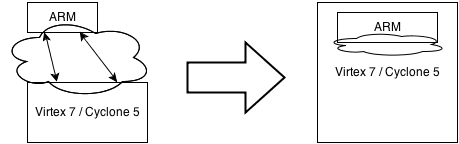
\includegraphics[width=2.5in]{socBlk.png}
\caption{Example of migration to embedded SoC FPGA}
\label{fig_socBlk}
\end{figure} 

\section{Project Overview}
Our original project proposal suggested using a framework called Open Crypto Framework (OCF)\cite{OCF2013}.  It turned out OCF was deprecated and not functional with newer Linux kernels.  Instead the Cryptodev development now provides a comparable capability along with a set of test applications used for validation and benchmarking.  This works out to fulfill the Crypto API and TestApp portions of the design.  The SHA1 entity is based on an Opencore core
.
As originally proposed, the architecture Figure \ref{fig_archBlkH} consists of a software kernel driver API, user space application, as well as a programmable logic (PL) entity.  Using these components, an initial implementation yielded a functional implementation of the SHA1 algorithm using the PL to compute the hash results.

\begin{figure}[ht]
\centering
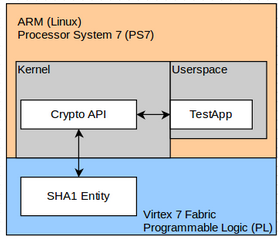
\includegraphics[width=2.5in]{highleveldesigndiagram.png}
\caption{High Level Design Architecture}
\label{fig_archBlkH}
\end{figure} 

\begin{figure}[ht]
\centering
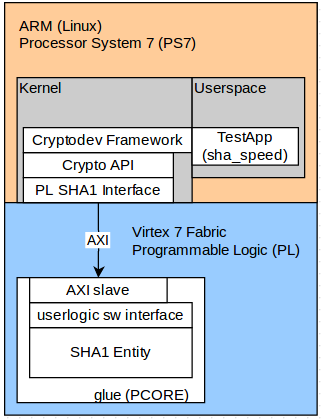
\includegraphics[width=2.5in]{lowleveldesigndiagram.png}
\caption{Detailed Design Architecture}
\label{fig_archBlkDetailed}
\end{figure} 

%\begin{figure}[ht]
%\centering
%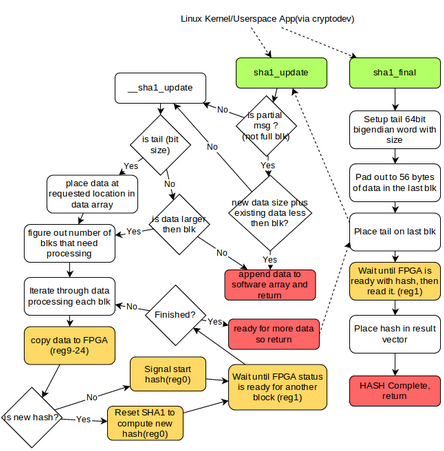
\includegraphics[width=2.5in]{softwareFlow.png}
%\caption{SHA-1 Flow Diagram}
%\label{fig_algoFlow}
%\end{figure} 

\section{Design Description}
The design consists of the components outlined in Figure \ref{fig_archBlkDetailed}.  Each of these is expanded in more detail in the sections that follow below.
\subsection{Hardware}
The Xilinx Zynq SoC FPGA 702 development kit was used as our target hardware. We acquired one development kit for our project and coordinated integration efforts to share the workload of only having one kit.  ISE tool support was included in the university's 14.6 license and the ISE EDK builder was used to pull together the embedded design. The Zynq ARM core Linux maturity was adequate in the Xilinx 14.6 release and Xilinx had some pretty good examples of interfacing between the fabric and processor. \cite{XIL2013} \cite{XILGNU2013}   The Zynq consists of two parts, the processing system 7 (PS7) and the programmable logic (PL). The PL might also be referred to as the “fabric” in the sections that follow.  The Zynq development kit was interfaced to via Ethernet and serial. With a base ARM load-set executing a Linux Kernel configured for modular development and capable of loading the PL images.
\subsection{Software}
For the software operating environment a full embedded Linux 3.12 Kernel and filesystem were used, allowing use of existing userspace applications and the Linux kernel’s existing infrastructure for cryptography.\cite{WIKPE2013} \cite{OCF2013} This configuration allowed the project to maximize reuse of the baseline algorithms already present in open source software and focus on gathering benchmark comparison data of our hardware accelerated approach.  The Xilinx Zynq board ARM OS load-set was based on Xilinx GIT tree source [14], with the Kernel/Rootfs being compiled into loadable binaries using the Buildroot \cite{BUILDROOT2013} embedded build system. We also added the Linux Cryptodev 1.6 support to the kernel and utilized the Cryptodev sha speed test app as part of our Buildroot rootfs.  The first stage bootloader (FSBL) was created using the Xilinx 14.6 EDK toolflow to export a XSDK FSBL project for our custom PL design.
\subsubsection{TestApp}
The test application used for executing the benchmarking of the baseline software algorithms on the SoC was based on the sha1\_speed application provided by the cryptodev-linux package.  It performed a number of block size test scenarios and captured throughput performance of each.

This application was also modified during integration (sha\_test) to allow generating of arbitrarily sized msg sizes to validate hash function behavior and buffer handling code.  It was also configured to send known msg sequences to validate against known hash results.  This was especially important when validating the behaviors were as expected between the single message and the multimessage scenarios (in multi-message the hash from the previous message is the seed to the next hash computation).
\subsubsection{Cryptodev Framework (Kernel Module)}
The Cryptodev framework’s linux device driver is designed to provide userspace applications access to Linux kernel crypto algorithms.  In our scenarios it’s used as is to provide initial test metrics against existing kernel software based algorithms.  As well as later it was used with the Zynq PL version of the SHA1 Opencore algorithm to run comparable test sequences to generate performance metrics.
\subsubsection{CryptoAPI (Kernel Interface)}
The kernel standard interface to all kernel crypto algorithms.  This was not modified as part of our project and instead a previous algorithm implemented was used as a template to help us conform to the existing Linux kernel Crypto API standard.
\subsubsection{PL SHA1 Interface Module}
The interface to the PL algorithm was implemented through a memory mapped set of registers (via a AXI interconnect to the PL).  The registers provided 32bit word access to control and status information.  They also provided the resulting hash and a method for data input.  The software interface code implemented a behavior that serviced the algorithm user logic entity based on register status feedback.  Currently the PL side of this interface does not use interrupts and requires the software to poll a register for status. 
 
This software interface received its data from the crypto API framework (Userspace --$>$ kernel) in blocks and then translated that data into what was needed to feed the SHA1 algorithm in the PL.  The diagram Appendix Figure C-1 shows the interactions between software and the PL.  The userspace TestApp would send data to the Cryptodev driver that would intern call the Kernel Crypto API that would call the sha1\_update function for each block of data.  When the last block is passed, the kernel API calls the sha1\_final.  In sha1\_final, the tail is appended before hashing the final bits of data.  Followed by the retrieval of the hash before the function returns.  
\subsection{Programmable Logic}
The Programmable Logic (PL) portion of our project consisted of three sub-components: (1) an AXI slave, (2) the SHA1 logic, and (3) a user-logic entity that implemented the register interface and interfaced with the SHA1 logic (user\_logic.vhd).  In addition to these three synthesized components, several simulation-only entities were created to verify the correctness of our design and to extract preliminary performance metrics.
Development of the PL entities were performed using the Xilinx 14.6 ISE/XPS tools.
Each of the main sub-components are explored in the following sub-sections.
\subsubsection{Glue (PCORE)}
As shown in Figure \ref{fig_archBlkDetailed}, an AXI bus connects the ARM core to the PL. The Xilinx CORE Generator System \cite{COREGEN} was used to create an AXI slave called 'glue' (glue.vhd).  We did not alter the generated 'glue' component for this project.
\begin{figure}[ht]
\centering
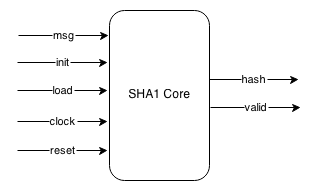
\includegraphics[width=2.5in]{Sha1_Core_Block_Diagram.png}
\caption{SHA-1 Core}
\label{fig_algoCore}
\end{figure} 
\subsubsection{SHA1 Core}
Our SHA1 core shown in Figure \ref{fig_algoCore} was based upon an open-source SHA1 core written by Arif Nugroho\cite{SHAOPEN}. After studying its implementation, we created a test-bench for the core (sha\_tb/sha1\_tb.vhd and sha\_tb/sha1\_tb\_driver.vhd) to both verify that it produced the correct hash results and to confirm our assumptions about its usage.

Starting from a working core saved us a great deal of development time. This particular core also had the distinct advantage of having no external dependencies beyond the standard IEEE libraries. However, the standalone nature of the core also posed several challenges. The core imposed strict timing requirements for both supplying message data and extracting the hash results. Loading sixteen words of message data into the core required a new word be supplied to the msg input signal every clock cycle for sixteen consecutive clock cycles. There was no way to delay message input. Similarly extracting the five word hash result required reading the hash signal for five consecutive clock cycles. The core user had exactly one clock cycle to begin capturing the hash results once the core's 'valid' signal became active.  Failure to do observe these requirements would produce incorrect hash results.

An even bigger challenge was the core's handling of multi-block messages. Each block consisted of sixteen words. Upon seeing the 'valid' signal become active, the user had to supply the next message block within eighty clock cycles. Owing to its design, there was no way to prevent the core from continuing to produce new hash values even if the user had not supplied new message values.

These challenges of SHA1 core were addressed in two ways. First, a FSM was added to the glue logic to insure the timing requirements for supplying message values and retrieving hash results were satisfied (see the next section). Secondly, the SHA1 core was modified to save a hash result only when new message data had previously been supplied.  This small modification to the core effectively stalled its progress until new data had been supplied by the user.
\subsubsection{User-logic SW Interface (PL)}
As discussed in the "PL SHA1 Interface Module" section, the PL SHA1 Interface software running on the ARM core expects to read and write to memory-mapped registers.  To achieve this capability, the Xilinx CORE Generator System was used to create the initial user\_logic component that defines those registers, and connects them to the AXI slave.  This user\_logic component was altered for this project to fit our requirements.  Specifically, it was modified to define behaviors for the different registers, and to define an FSM for interfacing with the SHA1 core. 

The initial (generated) user\_logic entity defined 32 general-purpose 32-bit registers that could be read and written by software.  For this project, we modified the user\_logic to give 23 of the registers specific roles.  One register was used to initiate a hash operation (ZYNQ\_SHA1\_RST), one register was used to report the status of the hash operation (ZYNQ\_SHA1\_STATUS), five registers were used to hold the hash value (ZYNQ\_SHA1\_H0-ZYNQ\_SHA1\_H4), and sixteen registers were used to each hold one 32-bit word of the 64-byte message block (ZYNQ\_SHA1\_D0-ZYNQ\_SHA1\_D15).  See Appendix Table C-1 for a complete register definition. 

One possible improvement would be to enhance the user\_logic entity to use interrupts to signal when the software should transition states.  This would reduce the overhead of bus transactions required to maintain status and free the ARM processor up to execute other tasks.  It would also slightly increase throughput as a few additional clock cycles might become available.
\begin{figure}[ht]
\centering
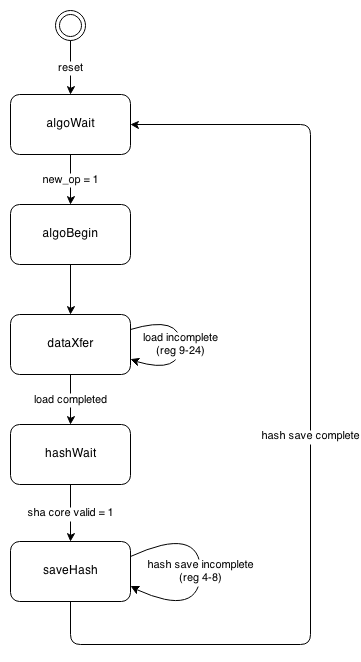
\includegraphics[width=2.5in]{UserLogicStateDiagram.png}
\caption{SHA-1 State Machine}
\label{fig_algoFSM}
\end{figure}
As discussed in the previous section, the slightly modified SHA1 core had specific timing requirements associated with supplying the message block and retrieving the hash results.  To accommodate these requirements a FSM called ‘user\_fsm’ was created as shown in Figure \ref{fig_algoFSM}.   This FSM idles in the ‘algoWait’ state until either a 1 value (hash new message block) or a 2 value (hash next message block) is written into the (unfortunately named) ‘rst’ register.  After proceeding through the ‘algoBegin’ state (discussed later), it then supplies 16 words of data into the SHA1 core from the corresponding user\_logic registers (dataXfer).  It then waits until the hash operation completes which is signaled when the SHA1 core raises the ‘valid’ signal (hashWait).  Once the hash is ready, it retrieves the five words of hash data from the core and stores them into the appropriate user\_logic registers (saveHash), before transitioning back to the ‘algoWait’ state.

One of the user\_logic design goals was to gracefully handle stale entries in the rst register.  Early version of user\_fsm would immediately begin a new round of hashing unless the software cleared the rst register soon after setting it.  Imposing this requirement on software was unacceptable.  At the same time, we wanted user\_logic to handle software that, for whatever reason, wrote the same value to the rst register over any number of cycles.  In both situations we wanted the user\_fsm to only begin a new round of hashing when software wrote a “fresh” 1 or 2 value to the rst register.

To accommodate both design goals, a new\_op signal was defined, and the user\_fsm was modified to only leave the algoWait state if new\_op was set.  The process that updated the rst register in response to AXI activity sets new\_op to 1 only when the rst register was NOT updated in the in the previous clock cycle or a different value was written to the rst register in the previous clock cycle.  This prior state history was maintained via two new signals updated each clock cycle: p\_reg\_write\_sel and p\_Bus2IP\_Data.  The new\_op signal was cleared when the user\_fsm transitioned to the ‘algoBegin’ state.

The overall operation of SHA1 PL design is shown in a flow diagram in the Appendix Figure C-1. All flow starts from the (top) userspace application running on the ARM.  The boxes in green are the kernel function calls that implement the custom SHA1 interfacing to the PL (sha1\_update/final as discussed in Section: “PL SHA1 Interface Module”).  The boxes in yellow are interactions with the PL register map (FSM).  The boxes in red are return/final states.  Bringing this all together, the diagram shows the software control access and PL status interactions, as well as the data load and hash retrieval steps.

\section{Experimental/Testing Results}
\subsection{Simulation}
\begin{figure}[ht]
\centering
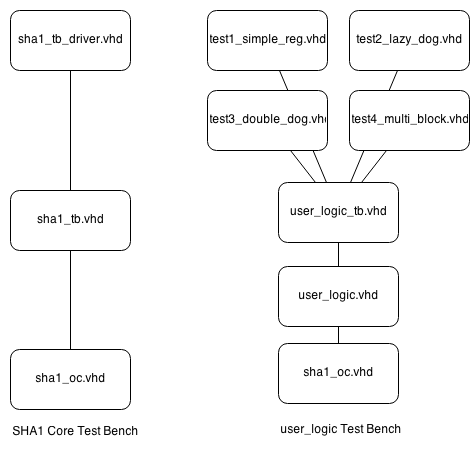
\includegraphics[width=2.5in]{Test_Benches.png}
\caption{Test bench coverage}
\label{fig_TB}
\end{figure} 
Our simulation effort for this project focused on two components: the open-source SHA1 core and the modified user\_logic component.  As outlined above, we simulated the SHA1 core to insure that it produced the correct hash results, to validate our understanding of the core’s operation and to confirm that stalling the core worked properly.  Simulation of the user\_logic component validated the proper functioning of the user\_fsm, and was also used to estimate overall performance and extract the relative amount of time spent in the primary user\_logic states (the yellow boxes in Appendix Figure C-1).

For each simulation effort a distinct test-bench was created as shown in Figure \ref{fig_TB}.  To make the user-logic test-bench more readily extend-able the logic was divided into a single generic “test-harness” component (user\_logic\_tb.vhd) , and a collection of individual test components.  The test-harness executed each test separately and performed a reset of the user\_logic logic prior to running the next test.  Tests consisted of validating the hash result of a single message block, multiple independent message blocks, and chained message blocks.  The Linux command-line tool ‘sha1sum’\cite{SHASUM}  was used to calculate the expected hash result for each of the test messages, and these hash results were further validated using online SHA1 calculators\cite{SHASUMONLINE}.

We decided not to create a test-bench for the processor interface level, since the AXI slave was a generated pcore.  We assumed that Xilinx would have performed the necessary validation of this logic and provided an optimal performing component.

The following subsections describe each of the user\_logic tests and present the performance metrics extracted from each.  Result data is detailed in Appendix A: Table A-1.
\subsubsection{Test1-Bus access}
\begin{figure}[ht]
\centering
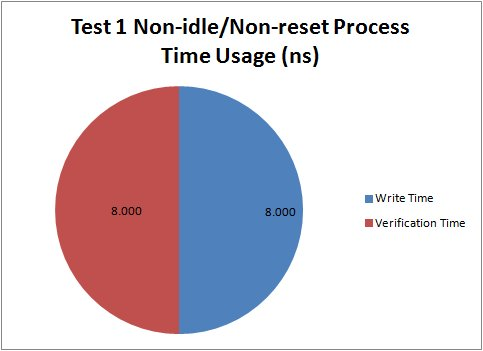
\includegraphics[width=2.5in]{Test1.jpg}
\caption{Test1 Runtime}
\label{fig_test1Runtime}
\end{figure} 
The initial simulation was used as a benchmark to give a metric as to the actual time it would take to write to and read from the FPGA after sufficient data had been received at the microprocessor.  Four bytes of data were written to the output registers, sent to the FPGA, and read back without encoding them.  The bytes were then compared with their initial values to verify there was no corruption.  An initial metric of 17 ns for overall process time, 8 ns for data transfer, 8 ns for verification, and 1 ns idle time was established to determine overhead per 4 bytes of data received as shown in Figure \ref{fig_test1Runtime}.  This step validated that the signals, registers, and encryption algorithm were working properly with the IP2Bus and provided a baseline for all other metrics.
\subsubsection{Test2 - Single block}
\begin{figure}[ht]
\centering
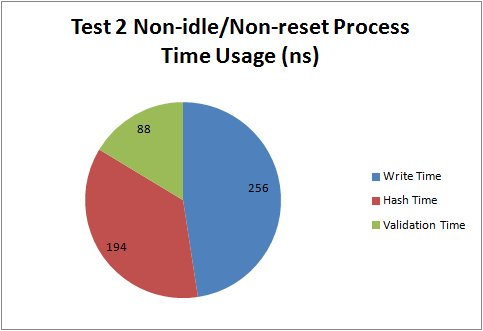
\includegraphics[width=2.5in]{Test2.jpg}
\caption{Test2 Runtime}
\label{fig_test2Runtime}
\end{figure} 
The second test in the simulation was to send 44 bytes of data through the SHA1 hash as a single block and validate the generated hash.  This test was set to validate an entire block of data passed through the SHA-1 core.  The write time increased disproportionately to the amount of data sent due to wait time in between writing to the registers and the passing of data to the SHA-1 core.  Hash time was added in for the time in hash process and the validation time increased proportionally to the amount of data sent.  See Appendix A: Table A-1 for detailed metrics used to create Figure \ref{fig_test2Runtime}.
\subsubsection{Test3 - Single block twice}
\begin{figure}[ht]
\centering
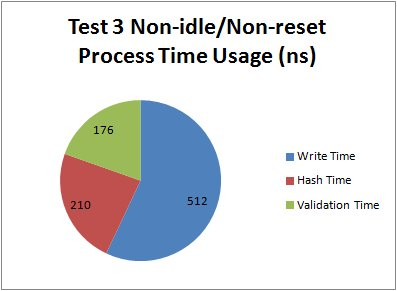
\includegraphics[width=2.5in]{Test3.jpg}
\caption{Test3 Runtime}
\label{fig_test3Runtime}
\end{figure}
The third test in the simulation was to send 44 bytes of data through SHA1 hash twice, each time computing a single block and validating the generated hash.  This test was set to validate the proper function of writing to the registers multiple times with a proper hash calculated with each block sent.  The write time and validation time doubled as expected while the hash time was optimized and showed a better performance than Test 2.  See Appendix A: Table A-1 for detailed metrics used to create Figure \ref{fig_test3Runtime}. 
\subsubsection{Test4 - Multi block}
\begin{figure}[ht]
\centering
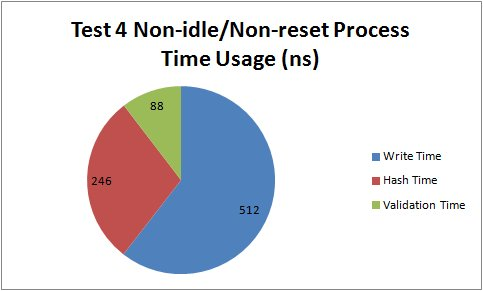
\includegraphics[width=2.5in]{Test4.jpg}
\caption{Test4 Runtime}
\label{fig_test4Runtime}
\end{figure} 
The fourth test in the simulation was to send 88 bytes of data through the SHA1 hash and have the algorithm process it as two blocks (multi-message).  This test was to validate the proper function of running multiple blocks through the SHA-1 core while maintaining an appended hash.  Write time stayed the same as expected while validation time was halved due to only one hash result needing to be verified, unlike Test 3.  Hash time only increased slightly and was due to the need to carry over the hash from the first block instead of the hard coded initial hash values.  See Appendix A: Table A-1 for detailed metrics used to create Figure \ref{fig_test4Runtime}.

The most noticeable sim performance observation was how the system was always in a state of feeding data.  This resulted in our limiting factor being the width/rate of the data bus used to send data to the FPGA.  If this data bus width/rate were increased so that more than one registers worth of data could be written or data written to individual registers at a faster pace, then more data could be processed in parallel on the FPGA.  

Another reality of the SHA1 algorithm was that it is inherently hard to speed up through parallelization (it being a sequential block hash).  You really instead end up counting instructions and optimizing the approach to supplying the data.  Compared to a non-block cipher that could easily be parallelized and accelerated using the method this project used. 
\subsection{Target Hardware}
1) For our first scenario we wanted to verify that our kernel, rootfs, and cryptodev kernel module were functional.  We cross built a kernel and rootfs with cryptodev support (kernel module and test apps), and then loaded them onto the sdcard and booted the Zynq board.  

Next, we executed the sha\_speed test and recorded the results.  The standard test sequence included loading the cryptodev kernel module to give us access to the Kernel Crypto APIs and the respective sha1\_asm or sha1\_zynq algorithm module.  
The kernel in this case was configured to use the default sha1\_arm hash algorithm, which is an ASM optimized implementation for ARM.  The results of this scenario are part of the graph under performance metrics (figure X).

2) The second scenario involved the start of the integration of the Linux Kernel Crypto API driver (sha1\_zynq).  This involved coding up a stubbed out PL interface behavior which allowed the software to go through it’s paces but without actually computing any hash.  Instead it just validated the data it was passed and some attempt was made to take the first stab at endian issues.  The TestApp was used to exercise this stubbed out driver.

3) The third scenario pulled together the integration of the Kernel driver software interface to an example glue pcore entity.  It validated the control/status register state-machine in the glue entity.  This scenario again used the TestApp (sha\_test) and exercised stubbed out known answers to validate behavior from userspace all the way to the pcore glue entity in the PL.

4) The fourth scenario performed the initial integration and checkout of a single block hash (the easy first case).  It validated the actual user-logic FSM used to interact with the SHA1 algorithm, it verified that the algorithm was resetting correctly between separate hash attempts, and clarified some endian issues.  This executed the TestApp and got our first performance numbers for msg sizes under 64bytes.

5) The fifth and last scenario pulled it all together with the multi-message (block) case.  It validated our buffering in the kernel driver was performing correctly and that the hash carry over in the algorithm entity was correct.   This executed the TestApp and got our performance metrics to compare with the original software baseline.

\section{Performance Metrics}
Our initial baseline metrics utilize a Linux Kernel SHA1 algorithm optimized using ARM assembly.  The same cryptodev framework and userspace test app were used in both the software and fabric scenarios.

The initial metrics were gathered for a generic software SHA1 and an ARM assembly optimized SHA1. 
\begin{figure}[ht]
\centering
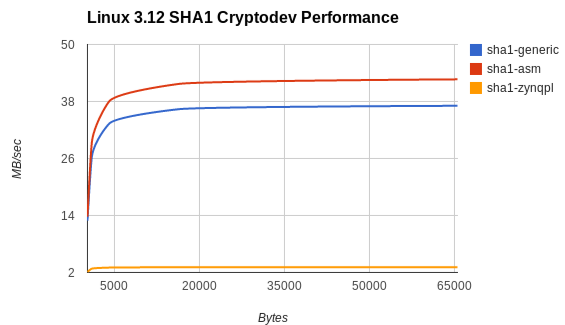
\includegraphics[width=3.5in]{perf.png}
\caption{SHA1 Cryptodev Performance}
\label{fig_algoPerf}
\end{figure} 
The performance of our Zynq PL based SHA1 implementation was significantly worse than a pure software based implementations as shown in Figure \ref{fig_algoPerf}. We believe the difference can be explained by our choice of algorithm, the clock advantage of the core, and our PL’s IO design. 

In retrospect, choosing the SHA-1 hash may have been a mistake.  There are two characteristics of this particular algorithm that make it a poor choice for use in reconfigurable hardware.  The first is that SHA-1 is inherently sequential.  Hashing a 64-byte block requires eighty iterations, with the results of each iteration feeding into the next.  Hashing multiple blocks follows a similar pattern (the result of one hash is used as the “seed” for the next).  The second characteristic is that the SHA-1 algorithm works on 32-bit words and uses the following commonly supported operations: ‘add’, ‘and’, ‘or’, ‘xor’, ‘rotate’, and ‘mod’. These data-sizes and operations are readily supported on all modern CPUs.  Without some form of parallelism or complex computation to perform, the FPGA design had very little in the algorithm to exploit.

The ARM core for our project ran at 667Mhz, while our PL design ran at a reference clock of 50Mhz.  A maximum of five 32-bit operations are performed each iteration of the SHA-1 hash.  While the FPGA could perform these operations in one clock cycle or 20ns, the ARM core could complete five operations in about 8ns.  The difference between the CPU’s clock speed and the PL’s was an order of magnitude.

Finally, our implementation of the SHA1 algorithm on the Zynq PL relied upon the CPU to supply it with data.  It had no mechanism to read memory directly.  This additional overhead of going through the CPU gives a distinct advantage to the pure software approach, which also has to read the hash message from memory, but then doesn’t have to redirect the data onto the slow(er) AXI bus in order to calculate the hash result.
\subsection{Future Enhancements}
There are a number of enhancements we could make to our PL design to potentially improve its performance.

One enhancement would be to add DMA capabilities to to our PL design, allowing it to read and write directly into memory.  Such an approach would eliminate all CPU instructions currently involved in loading and storing each piece of msg data from RAM to FPGA IO space.  It would also free the CPU to perform other work while the hash operation was proceeding.

Obviously, increasing the clock frequency of the AXI interface would allow us to supply data into the PL design faster.  It would also cause the hash calculations to complete sooner.

While the SHA-1 algorithm is inherently sequential, it should be possible to pipeline our PL design and improve overall hashing throughput.  The hashing operation can begin as soon as the first 32-bit word arrives.  The subsequent 15 iterations each consume one additional word of the message block.  Thereafter, an additional 64 iterations are performed during which time up to four other hash operations could be started.  We could potentially improve our hashing throughput by 5x.  Admittedly, even with a 5x improvement in throughput the pure software approach still performs better.

One final improvement would be to drop the SHA-1 hash altogether, and pick a hashing algorithm that is more amenable to parallelism or involves a complicated series of computations on usual data sizes.  Additional research into hash algorithms would be needed if this approach was taken.
\subsection{Runtime analysis of the AXI bus transactions}
The chipscope screenshots necessary for the following discussions have been captured in Appendix B. The first scenario captures the initial software status checking and loading of the data to be hashed  (Figure B-3).  The read valid signal was used to capture the initial software access to the status register (Figure B-2).  Initially, the (Figure B-3) shows the softwave time to determine to begin writing data took 50uSec from the time it initially read the status register noting that the algorithm was ready for data until the data actually hits the bus.  Next the complete software load of the data took 970uSec.  Then the software wrote a value of 0x1 to the control register to tell the user interface to begin processing the data.  At this point the capture ends (only had a buffer to view ~1.4uSec of transactions).  The time between when data is loaded and then the hash is computed is purely based on the algorithm compute time at 50Mhz characterized in simulation.

In the second scenario,   (Figure B-5) the read data value was used to trigger when the data read had a value of 0x7 signaling the hash computation in the algorithm entity is complete.  This capture provides the completion timeline of the software sequence to read out the computed hash result.  The software read the status register (0x4) until the status transitioned from a 0x7 to a 0x3.  This signaled the software to begin to read out the completed hash value (5 words) in ~230nSec.

Both of the scenarios captured for analysis seem reasonable based on the bus rates and a clock of 50Mhz.  The one possible area of growth they expose is the need to maximize the downtime while the intermediate hash compute is occurring in a multi-block hash.

The chipscope captures have been archived in our project repository under the chipscope folder.  We also included the cdc file and a chipscope setup file if it’s desired to actively review transactions.  The *.vcd files contain both an initial and final capture showing the software interfacing and algorithm entity inputs/outputs.  If a viewer is needed for the vcd files, we suggest http://www.iss-us.com/wavevcd/Wave\_msi.zip.  The setup file for this application is also checked in with our vcd files.  If the setup file doesn’t happen to work, open the respective vcd file and select the read/write address, data, and valids.  (They’re the signals with short names/labels.)

\section{Reproducing Results}
\subsection{Project Materials}
All of our project files submitted with this report are also stored in the following GIT repository (https://github.com/matthew-l-weber/cpre583\_pjt/).  The folder structure is separated into a folder for buildroot (ie the rootfs and kernel build system), a folder for our initial sha testbenches, a folder capturing our Chipscope files, and a folder for our toplevel XPS project that creates our Zynq image with the embedded pcore SHA1 module. 
\subsection{Simulation}
Software simulation was done on a Gnome Desktop, Red Hat, Linux system running Xilinx version 14.6 ISE and ModelSIM.  We used an emulator in bash mode and browse to the xpsTopLevelProj\_FinalProj/pcores/glue\_v1\_00\_a/devl/projnav folder in the files provided.  From here source the setup.sh file and then launch the ISE with the command ise glue.xise.  In ISE we verified all items were listed and have no conflicts.

To run the simulation and observe results we ran the behavioral model simulation on the  user\_logic\_tb - rtl (user\_logic\_tb.vhd) file by selecting the simulation radio button and double-clicking the Simulate Behavioral Model in the Processes listing.

The simulation ran in ModelSim with all four tests running consecutively over 3 microseconds with registers and wires being displayed in the waveform window.  Process times were measured using the timing in the waveform and running the processor frequency of 1 GHz. Detailed steps for running the simulation and the data results used for metrics are contained in Appendix A.

\subsection{Target Hardware}
The buildroot folder in our git repo consists of a couple configurations and overlays that can be used as follows to reproduce our SDcard image.  The first step is to do a git clone of buildroot on a Ubuntu 10.x or newer Linux machine.
	git clone git://git.buildroot.net/buildroot
Then copy the buildroot\_defconfig from our git's buildroot folder to the configs folder of the buildroot git clone.  Command buildroot to attempt to build that config as follows.

	\emph{make buildroot\_defconfig}
	
Then command it to extract the linux source for us to apply an overlay.

	\emph{make toolchain linux-extract}
	
Then copy over the linux folder from our git's buildroot folder into the output/build/ folder of the git clone.  Also copy over the linux.config file to the root of the git clone.  Next command buildroot to do a full build.

	\emph{make} 
	
This should successfully finish without errors.  Follow the following instructions to create an sdcard (http://www.wiki.xilinx.com/Prepare+Boot+Medium) and make sure to us the 14.6 release as the binary inputs.  Plus substitute the zImage they provide with the one built by buildroot (output/images) and ignore the initram fs that is in the Zynq release as our zImage includes the filesystem.  The filesystem includes the kernel module for the sha1\_zynq.ko and the sha\_speed test.  Once a valid bit file is generated by XPS there are two options to get it on the target.  The first is to copy it into the buildroot/output/targets folder and then command buildroot to “make linux-rebuild” which will repackage the zImage.  Then copy the new zImage over to the sdcard.  The other option is to remote to the Zynq board via SSH and SCP the file over.

In the root of the buildroot folder we included the final copies of all our boot images, test apps, kernel modules, and a copy of our initial/final test metrics.  The sha\_test app is our custom sha\_speed app that allows known pattern test cases.  The sha\_speed app is the stock cryptodev test app.

The xpsTopLevelProj\_FinalProj folder contains a XPS 14.6 project.  Within this project is an implementation folder with our resulting system.bit/bin file.  It also includes a pcores folder that has our sha1 module (testbenches and source), plus some AXI slave interface code.  The sha1 module is a separate ISE 14.6 project and the testbenches are executed at that project level.  The sha1 module pcore is incorporated by the toplevel XPS project as part of the overall system bit file generation.  The toplevel also adds in the chipscope AXI bus monitor that we used for analysis and integration.  Once the bit file is generated by the toplevel project, the bit file must be converted to a binary file for loading through Linux.  To do this, use the ISE promgen application with the args below or the python script (bit\_to\_zynq\_bin.py) which is checked in under the xps folders implementation folder.

\emph{Promgen -p bin -data\_width 32 -b -u 0x0 $<$ design\_name$>$.bit}

Then on the target a console is used to command the programming of the bit file.  This must be performed before any test scenarios are executed as a bad bus addressing may hang the AXI PL interface.
cat $<$project$>$.bit.bin $>$ /dev/xdevcfg

The chipscope folder contains the cpj file that saved our chipscope configuration.  The .cdc file captures our IO naming for the signals broken out.  We also included screen captures (Appendix B) detailing how to setup triggers and results from the start/finish of a hash sequence.  All the data captured was exported to vcd files and available for additional analysis using a waveform viewer tool mentioned in the performance metrics section above.

\section{Challenges and Obstacles}
One of the biggest challenges of this project was integrating the standalone SHA1 core into the Xilinx generated user\_logic component.  As discussed above, this required a thorough understanding of both components, along with the modifications and extensions to properly “glue” them together.  We anticipated that this effort might take time and budgeted an entire week to accomplish this task.

What we did not anticipate was the amount of time it took to merge one independently developed ISE project into another.  This simple task took five evenings to accomplish!  Only  through a combination of web-searches, posts on Blackboard, and trial-and-error did we   The fix was trivial once we had a better understanding of how ISE managed VHDL libraries, but getting to that understanding took web-searches, posts on Blackboard, and trial-and-error.  The real obstacle in this situation was our general lack of experience with Xilinx ISE and overall tool-flow.

In our original project proposal we expressed our intent to use a high-level synthesis tool to a convert a C implementation of the SHA-1 algorithm directly into VHDL.  We were then going to compare our hand-coded core against the synthesized version to determine how it compared in terms of performance and resource utilization.  In our proposal we listed two tools:  Xilinx HLS and Jacquard ROCCC 2.0.  in the course of working on this project we discovered that the university did not have a license for Xilinx HLS.  We were not inclined to purchase a license ourselves for a single project (about \$2000).  This left the ROCCC 2.0 compiler.  Although the ROCCC web-site is operational, the project itself appears to be either defunct or simply uninterested in responding to students.  All inquires to get a student license for the ROCCC 2.0 compiler went unanswered.
\section{Conclusion}
The implementation of a PL SHA1 cryptographic algorithm using the Linux kernel Crypto API showed to be successful.  With modifications to the user logic PL interface that would make the system custom to our application, integration of a SHA1 PL core, and tying it all together in simulation and on hardware.  In this process we thought that the core initially could operate with a lower process time if the state machine was driven by interrupts instead of process control to allow the software to execute parallel processes instead of waiting for data.  We did not explore this avenue as it was not in the scope of the project.  To test the system we stepped through a software simulated validation of the pieces with a final test on sending multiple block messages that gave successful data.  Upon examining the waveforms in the simulation we discovered the process time in the SHA-1 core could be optimized a bit more by using a wider AXI bus to send more than one 32 bit word at a time for more parallelized processing.
With a successful implementation of a software simulated SHA-1 we moved to a hardware implementation on a Zynq board.  We used the same approach as the software validation and stepped through tests to verify that all pieces were working properly with the final test being a multi block message being passed through the core and validated on the output.  This proved to be successful in the end, but has significant performance depreciation in speed.  We attributed this to the 50 MHz clock signal on the Zynq board and AXI bus to the ARM core while the software version ran a 1 GHz clock signal and all three pieces were in phase on the clock signal.  We achieved all middle level milestones for the project while discovering several areas for future development and extended data for this report.


\begin{thebibliography}{1}

 \bibitem{ALTERA2013}
Altera,
 \emph{Altera SoC Overview}.    
 http://www.altera.com/devices/processor/soc-fpga/overview/proc-soc-fpga.html, Oct 2013.

 \bibitem{ALTERA_NIOS2013}
Altera,
 \emph{Altera Nios Overview}.    
 http://www.altera.com/devices/processor/ nios2/ni2-index.html, Oct 2013.

 \bibitem{BUILDROOT2013}
Buildroot,
 \emph{Buildroot: making Embedded Linux easy}.    
 http://buildroot.uclibc.org/, Oct 2013.

 \bibitem{GAISLER2013}
Gaisler,
 \emph{Gaisler LEON Overview}.
 http://www.gaisler.com/index.php/ products/processors/leon3, Oct 2013.

 \bibitem{Kero2013}
Angelos Keromytis, Jason Wright, Theo Raadt
 \emph{The Design of the OpenBSD Cryptographic Framework}.    
 http://www.openbsd.org/papers/ocf.pdf, Proceedings of the USENIX Annual Technical Conference, pages 181-196, 2003.

 \bibitem{JACQUARD2013}
Jacquard,
 \emph{Riverside Optimizing Compiler for Configurable Computing}.    
 http://www.jacquardcomputing.com/roccc/, Oct 2013. 
  
 \bibitem{OCF2013}
David McCullough,
 \emph{Open Crypto Framework - Linux}.    
 http://ocf-linux.sourceforge.net/, Sept 2013.

 \bibitem{OPENSSL2013}
OpenSSL,
 \emph{OpenSSL}.    
 http://www.openssl.org/, 2013.

 \bibitem{TI2013}
Texas Instruments,
 \emph{Cryptography Users Guide}.    
 http://processors.wiki.ti.com/index.php/Cryptography\_Users\_Guide, Sept 2013.
 
 \bibitem{WIKPE2013}
Wikipedia,
 \emph{Crypto API Linux}.    
 http://en.wikipedia.org/wiki/ Crypto\_API\_(Linux), Oct 2013.

 \bibitem{XIL2013}
Xilinx,
 \emph{Xilinx Zynq All Programmable SoC}.    
 http://www.xilinx.com/products/silicon-devices/soc/zynq-7000/, Oct 2013.
 
 \bibitem{XILGNU2013}
Xilinx,
 \emph{Xilinx Zynq SoC Linux}.    
 http://www.xilinx.com/products/zynq-7000/linux.htm, Oct 2013.
 
 \bibitem{XILESL2013}
Xilinx,
 \emph{Xilinx Electronic System Level Design}.    
 http://www.xilinx.com/products/design-tools/vivado/integration/esl-design/index.htm, Oct 2013.
 
 \bibitem{XILSRC2013}
Xilinx,
 \emph{Xilinx GIT Repo}.    
 https://github.com/xilinx, Oct 2013.
 
\bibitem{ROCCC}J. Villarreal, A. Park, W. Najjar, and R. Halstead.
\emph{Designing modular hardware accelerators in C with ROCCC 2.0.}
In\emph{ Field-Programmable Custom Computing Machines (FCCM), 2010
18th IEEE Annual International Symposium, }2010\emph{.}

\bibitem{HIPPA}HIPAA Collaborative of Wisconsin, HIPAA Encryption
Whitepaper 7.7.10, http://www.general-files.org/download/gs584dd455h32i0/ encryption\%20whitepaper\%207.7.10.doc.html

\bibitem{IEEESTD}IEEE 1363-2000: Standard Specifications For Public
Key Cryptography, http://grouper.ieee.org/groups/1363/P1363/index.html

\bibitem{GUTMANN}Peter Gutmann, An Open-source Cryptographic Coprocessor,
University of Auckland, New Zealandhttp://www.cypherpunks.to/\textasciitilde{}peter/usenix00.pdf

\bibitem{GUERON}Shay Gueron, Vlad Krasnov; Parallelzing message schedules
to accelerate the computations of hash functions; Department of Mathematics,
University of Haifa, Isreal; June 5, 2012

\bibitem{SHASUM}
 \emph{SHA1 Summary Definition}
 http://linuxcommand.org/man\_pages/ sha1sum1.html
 
\bibitem{SHASUMONLINE}
 \emph{SHA1 Online Calculator}
 http://sha1-hash-online.waraxe.us/ 
 
\bibitem{SHAOPEN} 
 \emph{SHA1 Opencore}
 http://opencores.org/websvn,filedetails? repname=nfhc\&path=\%2Fnfhc\%2Ftrunk\%2Fsha1\%2Fsha1.vhdl

\bibitem{COREGEN} 
\emph{Xilinx Core Generator}
 http://www.xilinx.com/tools/coregen.htm

\end{thebibliography}

\end{document}
